\chapter{Tutorial para execução dos \textit{scripts Python} desenvolvidos para análise}
\label{cap:ap-tutorial}

Toda a análise realizada neste estudo foi implementada em linguagem
\textit{Python}, em sistema \textit{GNU/Linux Ubuntu}, utilizando
ferramentas de \textit{software livre}. O código-fonte, assim como
todo o conteúdo usado e gerado, encontra-se distribuído nos seguintes
repositórios abertos:

\begin{itemize}
  \item{\url{http://github.com/automata/dissertacao-ifsc}: contém o
    código-fonte \LaTeX \, desta dissertação e pode ser compilado através
    do comando \textit{make}, gerando um arquivo
    \textit{dissertacao.pdf} como saída.}
  \item{\url{http://github.com/automata/viz-paintings}: aplicativo Web
    desenvolvido em \textit{JavaScript} para visualização interativa
    da Figura~\ref{fig:caso1_g1}, onde o espaço de atributos pode ser
    ``navegado'' com \textit{panning} e \textit{zoom}, facilitando a
    identificação de cada pintura analisada e seu respectivo
    \textit{cluster}. Essa mesma aplicação pode ser acessada
    \textit{on-line} através do endereço
    \url{http://automata.github.io/viz-paintings}. Mais detalhes e
    capturas de tela do aplicativo no Apêndice~\ref{ap:alternativa}.}
  \item{\url{http://github.com/automata/tri-delaunay}: código-fonte em
    \textit{Python} para geração de pinturas generativas baseadas em
    figuras usadas neste estudo e triangulação de Delaunay. Estas
    pinturas foram exibidas em uma exposição em 2013
    (Apêndice~\ref{ap:sifisc}).}
  \item{\url{http://github.com/automata/ana-pintores}: \textit{scripts
      Python} usados para obter os resultados discutidos nesse estudo,
    assim como a base de figuras das 240 pinturas utilizadas. A
    seguir, instruções para instalação e uso de tais
    \textit{scripts}.}
\end{itemize}

\begin{enumerate}
  \item Certifique-se de ter instalado as dependências:
\begin{verbatim}
   sudo apt-get install python python-numpy python-matplotlib
                        python-setuptools git
   sudo easy_install scikit-learn
   git clone https://github.com/scikit-image/scikit-image.git
   cd scikit-image
   sudo python setup.py install
\end{verbatim}
  \item Clone o repositório Git da dissertação e \textit{scripts} (o repositório
    inclui os arquivos de imagens das pinturas, portanto o tempo de
    \textit{download} pode ser longo):
\begin{verbatim}
  git clone https://github.com/automata/ana-pintores.git
  cd ana-pintores/
\end{verbatim}
  \item Para analisar as pinturas por processamento de imagens, execute:
\begin{verbatim}
  python analise_pinturas.py
  python analise_segs.py
\end{verbatim}
  \item Para gerar a matriz de atributos extraídos a partir da análise anterior:
\begin{verbatim}
  python feature_matrix_gen.py
\end{verbatim}
  \item Para calcular as medidas de inovação, oposição e dialética, assim como
    plotar a série temporal considerando os dois melhores atributos e LDA, assim
    como uma versão alternativa que substitui os marcadores por miniaturas das
    pinturas:
\begin{verbatim}
  python metrics_caso1.py
  python metrics_caso3b.py
  python metrics_caso1_alternativo.py
\end{verbatim}
  \item Para validar os resultads através do LDA:
\begin{verbatim}
  python valida3_r.py
\end{verbatim}
  \item Para calcular as matrizes esparsas e o índice $\alpha$ de separação,
    listando e plotando os pares de atributos que apresentaram melhor separação: 
\begin{verbatim}
  python scatter_matrix_pintores.py
\end{verbatim}
  \item Para plotar o comparativo dos histogramas de níveis de cinza médio das pinturas:
\begin{verbatim}
  python chiaroscuro.py
  python chiaroscuro_modernos.py
\end{verbatim}
\end{enumerate}

Cada script produz arquivos de imagens e resultados de saída diversos. Seus
respectivos códigos devem ser consultados para se compreender quais as saídas
geradas.

%% \lstinputlisting[language=Python, label=codigo:analise_pinturas.py,
%%   caption=Analisa pinturas]{analise_pinturas.py}

%% \lstinputlisting[language=Python, label=codigo:analise_segs.py, caption=Analisa
%% pinturas segmentadas]{analise_segs.py}

%% \lstinputlisting[language=Python, label=codigo:feature_matrix_gen.py,
%%   caption=Cria a matriz de atributos a partir das análises]{feature_matrix_gen.py}

%% \lstinputlisting[language=Python, label=codigo:scatter_matrix_pintores.py,
%%   caption=Seleção de atributos por matrizes esparsas]{scatter_matrix_pintores.py}

%% \lstinputlisting[language=Python, label=codigo:metrics_caso3b.py,
%%   caption={Cálculo das medidas de oposição, inovação e dialética}]{metrics_caso3b.py}

%% \lstinputlisting[language=Python, label=codigo:matrix_confusao.py,
%%   caption=Validação do LDA por matriz de confusão]{matrix_confusao.py}

%% \lstinputlisting[language=Python, label=codigo:chiaroscuro.py,
%%   caption=Validação da influência estética em termos de contraste de Caravaggio
%%   em Velazquez e Vermeer]{chiaroscuro.py}

%% \lstinputlisting[language=Python, label=codigo:chiaroscuro_modernos.py,
%%   caption=Validação da individualidade estética em termos de contraste para os
%%   pintores modernos]{chiaroscuro_modernos.py}


\chapter{Galeria de imagens das 240 pinturas analisadas}
\label{cap:ap-galeria}

\begin{figure}[htb]
\centering \subfloat{%
  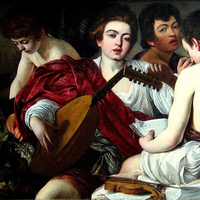
\includegraphics[width=.24\textwidth]{figs/thumbs/caravaggio/0}}\hfill \subfloat{%
  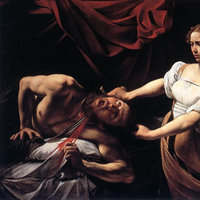
\includegraphics[width=.24\textwidth]{figs/thumbs/caravaggio/1}}\hfill \subfloat{%
  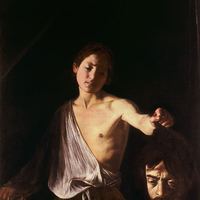
\includegraphics[width=.24\textwidth]{figs/thumbs/caravaggio/2}}\hfill \subfloat{%
  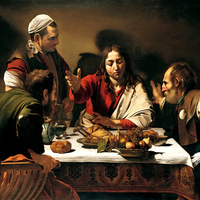
\includegraphics[width=.24\textwidth]{figs/thumbs/caravaggio/3}}\\ \subfloat{%
  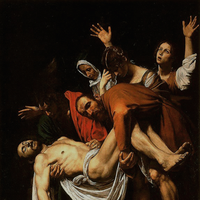
\includegraphics[width=.24\textwidth]{figs/thumbs/caravaggio/4}}\hfill \subfloat{%
  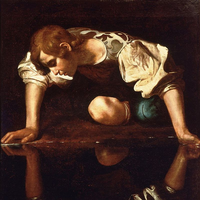
\includegraphics[width=.24\textwidth]{figs/thumbs/caravaggio/5}}\hfill \subfloat{%
  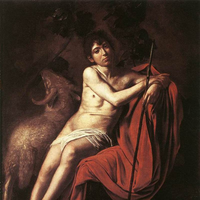
\includegraphics[width=.24\textwidth]{figs/thumbs/caravaggio/6}}\hfill \subfloat{%
  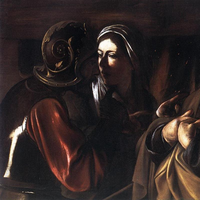
\includegraphics[width=.24\textwidth]{figs/thumbs/caravaggio/7}}\\ \subfloat{%
  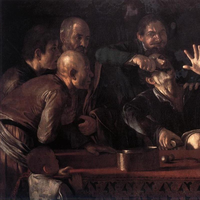
\includegraphics[width=.24\textwidth]{figs/thumbs/caravaggio/8}}\hfill \subfloat{%
  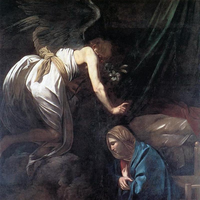
\includegraphics[width=.24\textwidth]{figs/thumbs/caravaggio/9}}\hfill \subfloat{%
  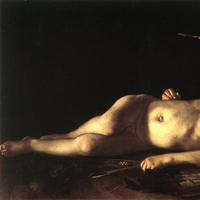
\includegraphics[width=.24\textwidth]{figs/thumbs/caravaggio/10}}\hfill \subfloat{%
  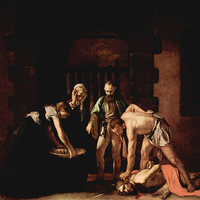
\includegraphics[width=.24\textwidth]{figs/thumbs/caravaggio/11}}\\ \subfloat{%
  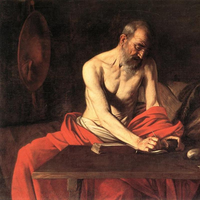
\includegraphics[width=.24\textwidth]{figs/thumbs/caravaggio/12}}\hfill \subfloat{%
  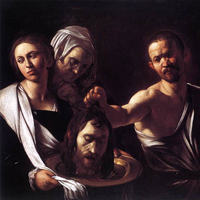
\includegraphics[width=.24\textwidth]{figs/thumbs/caravaggio/13}}\hfill \subfloat{%
  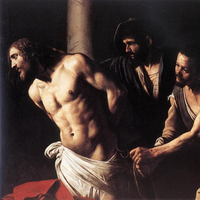
\includegraphics[width=.24\textwidth]{figs/thumbs/caravaggio/14}}\hfill \subfloat{%
  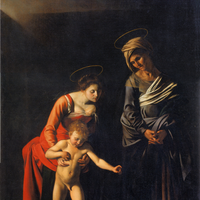
\includegraphics[width=.24\textwidth]{figs/thumbs/caravaggio/15}} \\ \subfloat{%
  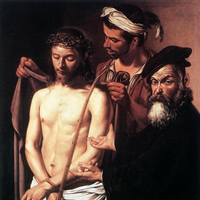
\includegraphics[width=.24\textwidth]{figs/thumbs/caravaggio/16}}\hfill \subfloat{%
  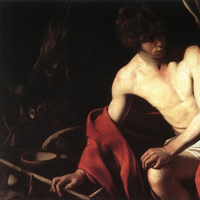
\includegraphics[width=.24\textwidth]{figs/thumbs/caravaggio/17}}\hfill \subfloat{%
  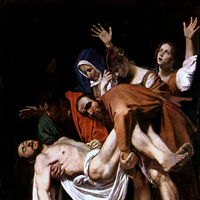
\includegraphics[width=.24\textwidth]{figs/thumbs/caravaggio/18}}\hfill \subfloat{%
  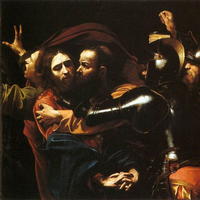
\includegraphics[width=.24\textwidth]{figs/thumbs/caravaggio/19}} \\

  \caption{Caravaggio}
  \label{fig:caravaggio_1}
\end{figure}

%% Frans Hals

\begin{figure}[htb]
\centering
  \subfloat{%
    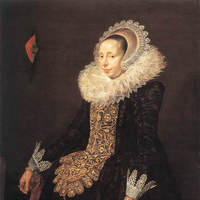
\includegraphics[width=.24\textwidth]{figs/thumbs/hals/0}}\hfill
  \subfloat{%
    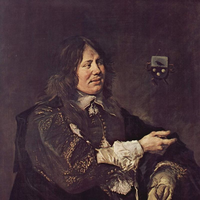
\includegraphics[width=.24\textwidth]{figs/thumbs/hals/1}}\hfill
  \subfloat{%
    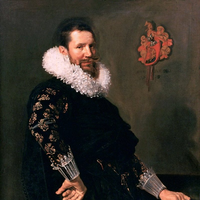
\includegraphics[width=.24\textwidth]{figs/thumbs/hals/2}}\hfill
  \subfloat{%
    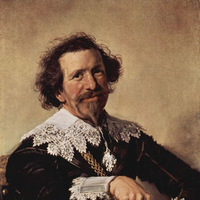
\includegraphics[width=.24\textwidth]{figs/thumbs/hals/3}}\\
  \subfloat{%
    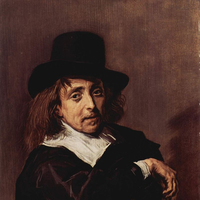
\includegraphics[width=.24\textwidth]{figs/thumbs/hals/4}}\hfill
  \subfloat{%
    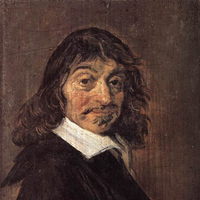
\includegraphics[width=.24\textwidth]{figs/thumbs/hals/5}}\hfill
  \subfloat{%
    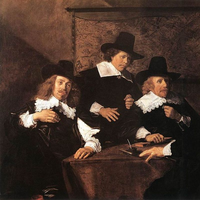
\includegraphics[width=.24\textwidth]{figs/thumbs/hals/6}}\hfill
  \subfloat{%
    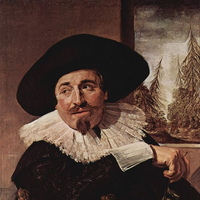
\includegraphics[width=.24\textwidth]{figs/thumbs/hals/7}}\\
  \subfloat{%
    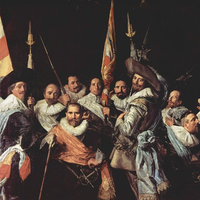
\includegraphics[width=.24\textwidth]{figs/thumbs/hals/8}}\hfill
  \subfloat{%
    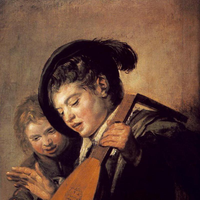
\includegraphics[width=.24\textwidth]{figs/thumbs/hals/9}}\hfill
  \subfloat{%
    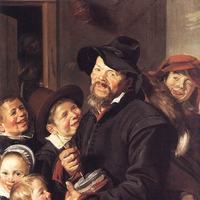
\includegraphics[width=.24\textwidth]{figs/thumbs/hals/10}}\hfill
  \subfloat{%
    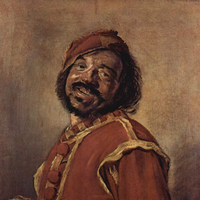
\includegraphics[width=.24\textwidth]{figs/thumbs/hals/11}}\\
  \subfloat{%
    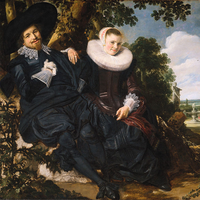
\includegraphics[width=.24\textwidth]{figs/thumbs/hals/12}}\hfill
  \subfloat{%
    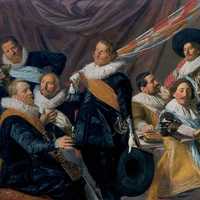
\includegraphics[width=.24\textwidth]{figs/thumbs/hals/13}}\hfill
  \subfloat{%
    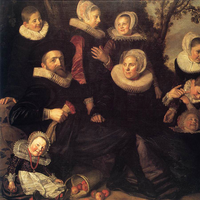
\includegraphics[width=.24\textwidth]{figs/thumbs/hals/14}}\hfill
  \subfloat{%
    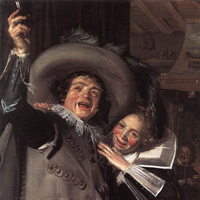
\includegraphics[width=.24\textwidth]{figs/thumbs/hals/15}} \\
  \subfloat{%
    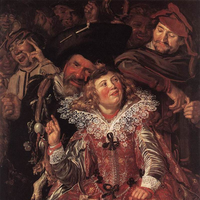
\includegraphics[width=.24\textwidth]{figs/thumbs/hals/16}}\hfill
  \subfloat{%
    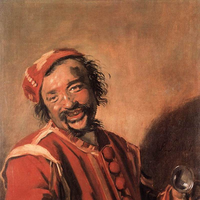
\includegraphics[width=.24\textwidth]{figs/thumbs/hals/17}}\hfill
  \subfloat{%
    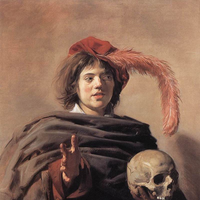
\includegraphics[width=.24\textwidth]{figs/thumbs/hals/18}}\hfill
  \subfloat{%
    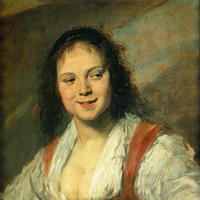
\includegraphics[width=.24\textwidth]{figs/thumbs/hals/19}} \\

  \caption{Frans Hals}
  \label{fig:hals_1}
\end{figure}

%% Nicolas Poussin

\begin{figure}[htb]
\centering
  \subfloat{%
    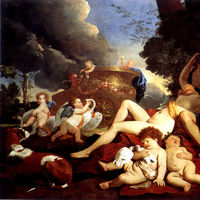
\includegraphics[width=.24\textwidth]{figs/thumbs/poussin/0}}\hfill
  \subfloat{%
    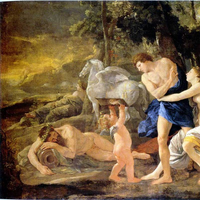
\includegraphics[width=.24\textwidth]{figs/thumbs/poussin/1}}\hfill
  \subfloat{%
    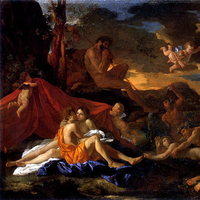
\includegraphics[width=.24\textwidth]{figs/thumbs/poussin/2}}\hfill
  \subfloat{%
    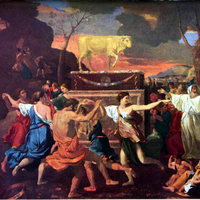
\includegraphics[width=.24\textwidth]{figs/thumbs/poussin/3}}\\
  \subfloat{%
    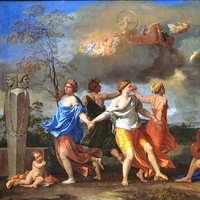
\includegraphics[width=.24\textwidth]{figs/thumbs/poussin/4}}\hfill
  \subfloat{%
    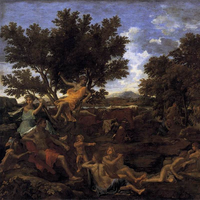
\includegraphics[width=.24\textwidth]{figs/thumbs/poussin/5}}\hfill
  \subfloat{%
    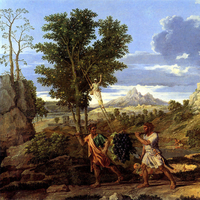
\includegraphics[width=.24\textwidth]{figs/thumbs/poussin/6}}\hfill
  \subfloat{%
    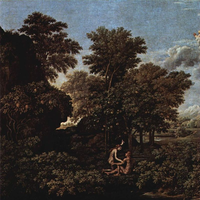
\includegraphics[width=.24\textwidth]{figs/thumbs/poussin/7}}\\
  \subfloat{%
    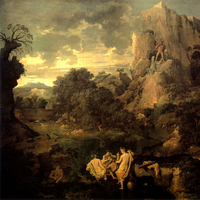
\includegraphics[width=.24\textwidth]{figs/thumbs/poussin/8}}\hfill
  \subfloat{%
    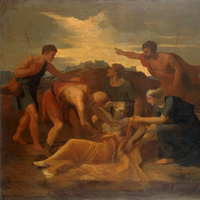
\includegraphics[width=.24\textwidth]{figs/thumbs/poussin/9}}\hfill
  \subfloat{%
    \includegraphics[width=.24\textwidth]{figs/thumbs/poussin/10}}\hfill
  \subfloat{%
    \includegraphics[width=.24\textwidth]{figs/thumbs/poussin/11}}\\
  \subfloat{%
    \includegraphics[width=.24\textwidth]{figs/thumbs/poussin/12}}\hfill
  \subfloat{%
    \includegraphics[width=.24\textwidth]{figs/thumbs/poussin/13}}\hfill
  \subfloat{%
    \includegraphics[width=.24\textwidth]{figs/thumbs/poussin/14}}\hfill
  \subfloat{%
    \includegraphics[width=.24\textwidth]{figs/thumbs/poussin/15}} \\
  \subfloat{%
    \includegraphics[width=.24\textwidth]{figs/thumbs/poussin/16}}\hfill
  \subfloat{%
    \includegraphics[width=.24\textwidth]{figs/thumbs/poussin/17}}\hfill
  \subfloat{%
    \includegraphics[width=.24\textwidth]{figs/thumbs/poussin/18}}\hfill
  \subfloat{%
    \includegraphics[width=.24\textwidth]{figs/thumbs/poussin/19}} \\

  \caption{Nicolas Poussin}
  \label{fig:poussin_1}
\end{figure}

%% Diego Velázquez

\begin{figure}[htb]
\centering
  \subfloat{%
    \includegraphics[width=.24\textwidth]{figs/thumbs/velazquez/0}}\hfill
  \subfloat{%
    \includegraphics[width=.24\textwidth]{figs/thumbs/velazquez/1}}\hfill
  \subfloat{%
    \includegraphics[width=.24\textwidth]{figs/thumbs/velazquez/2}}\hfill
  \subfloat{%
    \includegraphics[width=.24\textwidth]{figs/thumbs/velazquez/3}}\\
  \subfloat{%
    \includegraphics[width=.24\textwidth]{figs/thumbs/velazquez/4}}\hfill
  \subfloat{%
    \includegraphics[width=.24\textwidth]{figs/thumbs/velazquez/5}}\hfill
  \subfloat{%
    \includegraphics[width=.24\textwidth]{figs/thumbs/velazquez/6}}\hfill
  \subfloat{%
    \includegraphics[width=.24\textwidth]{figs/thumbs/velazquez/7}}\\
  \subfloat{%
    \includegraphics[width=.24\textwidth]{figs/thumbs/velazquez/8}}\hfill
  \subfloat{%
    \includegraphics[width=.24\textwidth]{figs/thumbs/velazquez/9}}\hfill
  \subfloat{%
    \includegraphics[width=.24\textwidth]{figs/thumbs/velazquez/10}}\hfill
  \subfloat{%
    \includegraphics[width=.24\textwidth]{figs/thumbs/velazquez/11}}\\
  \subfloat{%
    \includegraphics[width=.24\textwidth]{figs/thumbs/velazquez/12}}\hfill
  \subfloat{%
    \includegraphics[width=.24\textwidth]{figs/thumbs/velazquez/13}}\hfill
  \subfloat{%
    \includegraphics[width=.24\textwidth]{figs/thumbs/velazquez/14}}\hfill
  \subfloat{%
    \includegraphics[width=.24\textwidth]{figs/thumbs/velazquez/15}} \\
  \subfloat{%
    \includegraphics[width=.24\textwidth]{figs/thumbs/velazquez/16}}\hfill
  \subfloat{%
    \includegraphics[width=.24\textwidth]{figs/thumbs/velazquez/17}}\hfill
  \subfloat{%
    \includegraphics[width=.24\textwidth]{figs/thumbs/velazquez/18}}\hfill
  \subfloat{%
    \includegraphics[width=.24\textwidth]{figs/thumbs/velazquez/19}} \\

  \caption{Diego Velázquez}
  \label{fig:velazquez_1}
\end{figure}

%% Rembrandt

\begin{figure}[htb]
\centering
  \subfloat{%
    \includegraphics[width=.24\textwidth]{figs/thumbs/rembrandt/0}}\hfill
  \subfloat{%
    \includegraphics[width=.24\textwidth]{figs/thumbs/rembrandt/1}}\hfill
  \subfloat{%
    \includegraphics[width=.24\textwidth]{figs/thumbs/rembrandt/2}}\hfill
  \subfloat{%
    \includegraphics[width=.24\textwidth]{figs/thumbs/rembrandt/3}}\\
  \subfloat{%
    \includegraphics[width=.24\textwidth]{figs/thumbs/rembrandt/4}}\hfill
  \subfloat{%
    \includegraphics[width=.24\textwidth]{figs/thumbs/rembrandt/5}}\hfill
  \subfloat{%
    \includegraphics[width=.24\textwidth]{figs/thumbs/rembrandt/6}}\hfill
  \subfloat{%
    \includegraphics[width=.24\textwidth]{figs/thumbs/rembrandt/7}}\\
  \subfloat{%
    \includegraphics[width=.24\textwidth]{figs/thumbs/rembrandt/8}}\hfill
  \subfloat{%
    \includegraphics[width=.24\textwidth]{figs/thumbs/rembrandt/9}}\hfill
  \subfloat{%
    \includegraphics[width=.24\textwidth]{figs/thumbs/rembrandt/10}}\hfill
  \subfloat{%
    \includegraphics[width=.24\textwidth]{figs/thumbs/rembrandt/11}}\\
  \subfloat{%
    \includegraphics[width=.24\textwidth]{figs/thumbs/rembrandt/12}}\hfill
  \subfloat{%
    \includegraphics[width=.24\textwidth]{figs/thumbs/rembrandt/13}}\hfill
  \subfloat{%
    \includegraphics[width=.24\textwidth]{figs/thumbs/rembrandt/14}}\hfill
  \subfloat{%
    \includegraphics[width=.24\textwidth]{figs/thumbs/rembrandt/15}} \\
  \subfloat{%
    \includegraphics[width=.24\textwidth]{figs/thumbs/rembrandt/16}}\hfill
  \subfloat{%
    \includegraphics[width=.24\textwidth]{figs/thumbs/rembrandt/17}}\hfill
  \subfloat{%
    \includegraphics[width=.24\textwidth]{figs/thumbs/rembrandt/18}}\hfill
  \subfloat{%
    \includegraphics[width=.24\textwidth]{figs/thumbs/rembrandt/19}} \\

  \caption{Rembrandt Harmenszoon van Rijn}
  \label{fig:rembrandt_1}
\end{figure}

%% Johannes Vermeer

\begin{figure}[htb]
\centering
  \subfloat{%
    \includegraphics[width=.24\textwidth]{figs/thumbs/vermeer/0}}\hfill
  \subfloat{%
    \includegraphics[width=.24\textwidth]{figs/thumbs/vermeer/1}}\hfill
  \subfloat{%
    \includegraphics[width=.24\textwidth]{figs/thumbs/vermeer/2}}\hfill
  \subfloat{%
    \includegraphics[width=.24\textwidth]{figs/thumbs/vermeer/3}}\\
  \subfloat{%
    \includegraphics[width=.24\textwidth]{figs/thumbs/vermeer/4}}\hfill
  \subfloat{%
    \includegraphics[width=.24\textwidth]{figs/thumbs/vermeer/5}}\hfill
  \subfloat{%
    \includegraphics[width=.24\textwidth]{figs/thumbs/vermeer/6}}\hfill
  \subfloat{%
    \includegraphics[width=.24\textwidth]{figs/thumbs/vermeer/7}}\\
  \subfloat{%
    \includegraphics[width=.24\textwidth]{figs/thumbs/vermeer/8}}\hfill
  \subfloat{%
    \includegraphics[width=.24\textwidth]{figs/thumbs/vermeer/9}}\hfill
  \subfloat{%
    \includegraphics[width=.24\textwidth]{figs/thumbs/vermeer/10}}\hfill
  \subfloat{%
    \includegraphics[width=.24\textwidth]{figs/thumbs/vermeer/11}}\\
  \subfloat{%
    \includegraphics[width=.24\textwidth]{figs/thumbs/vermeer/12}}\hfill
  \subfloat{%
    \includegraphics[width=.24\textwidth]{figs/thumbs/vermeer/13}}\hfill
  \subfloat{%
    \includegraphics[width=.24\textwidth]{figs/thumbs/vermeer/14}}\hfill
  \subfloat{%
    \includegraphics[width=.24\textwidth]{figs/thumbs/vermeer/15}} \\
  \subfloat{%
    \includegraphics[width=.24\textwidth]{figs/thumbs/vermeer/16}}\hfill
  \subfloat{%
    \includegraphics[width=.24\textwidth]{figs/thumbs/vermeer/17}}\hfill
  \subfloat{%
    \includegraphics[width=.24\textwidth]{figs/thumbs/vermeer/18}}\hfill
  \subfloat{%
    \includegraphics[width=.24\textwidth]{figs/thumbs/vermeer/19}} \\

  \caption{Johannes Vermeer}
  \label{fig:vermeer_1}
\end{figure}

%% Vincent van Gogh

\begin{figure}[htb]
\centering
  \subfloat{%
    \includegraphics[width=.24\textwidth]{figs/thumbs/gogh/0}}\hfill
  \subfloat{%
    \includegraphics[width=.24\textwidth]{figs/thumbs/gogh/1}}\hfill
  \subfloat{%
    \includegraphics[width=.24\textwidth]{figs/thumbs/gogh/2}}\hfill
  \subfloat{%
    \includegraphics[width=.24\textwidth]{figs/thumbs/gogh/3}}\\
  \subfloat{%
    \includegraphics[width=.24\textwidth]{figs/thumbs/gogh/4}}\hfill
  \subfloat{%
    \includegraphics[width=.24\textwidth]{figs/thumbs/gogh/5}}\hfill
  \subfloat{%
    \includegraphics[width=.24\textwidth]{figs/thumbs/gogh/6}}\hfill
  \subfloat{%
    \includegraphics[width=.24\textwidth]{figs/thumbs/gogh/7}}\\
  \subfloat{%
    \includegraphics[width=.24\textwidth]{figs/thumbs/gogh/8}}\hfill
  \subfloat{%
    \includegraphics[width=.24\textwidth]{figs/thumbs/gogh/9}}\hfill
  \subfloat{%
    \includegraphics[width=.24\textwidth]{figs/thumbs/gogh/10}}\hfill
  \subfloat{%
    \includegraphics[width=.24\textwidth]{figs/thumbs/gogh/11}}\\
  \subfloat{%
    \includegraphics[width=.24\textwidth]{figs/thumbs/gogh/12}}\hfill
  \subfloat{%
    \includegraphics[width=.24\textwidth]{figs/thumbs/gogh/13}}\hfill
  \subfloat{%
    \includegraphics[width=.24\textwidth]{figs/thumbs/gogh/14}}\hfill
  \subfloat{%
    \includegraphics[width=.24\textwidth]{figs/thumbs/gogh/15}} \\
  \subfloat{%
    \includegraphics[width=.24\textwidth]{figs/thumbs/gogh/16}}\hfill
  \subfloat{%
    \includegraphics[width=.24\textwidth]{figs/thumbs/gogh/17}}\hfill
  \subfloat{%
    \includegraphics[width=.24\textwidth]{figs/thumbs/gogh/18}}\hfill
  \subfloat{%
    \includegraphics[width=.24\textwidth]{figs/thumbs/gogh/19}} \\

  \caption{Vincent van Gogh}
  \label{fig:gogh_1}
\end{figure}

%% Wassilly Kandinsky

\begin{figure}[htb]
\centering
  \subfloat{%
    \includegraphics[width=.24\textwidth]{figs/thumbs/kandinsky/0}}\hfill
  \subfloat{%
    \includegraphics[width=.24\textwidth]{figs/thumbs/kandinsky/1}}\hfill
  \subfloat{%
    \includegraphics[width=.24\textwidth]{figs/thumbs/kandinsky/2}}\hfill
  \subfloat{%
    \includegraphics[width=.24\textwidth]{figs/thumbs/kandinsky/3}}\\
  \subfloat{%
    \includegraphics[width=.24\textwidth]{figs/thumbs/kandinsky/4}}\hfill
  \subfloat{%
    \includegraphics[width=.24\textwidth]{figs/thumbs/kandinsky/5}}\hfill
  \subfloat{%
    \includegraphics[width=.24\textwidth]{figs/thumbs/kandinsky/6}}\hfill
  \subfloat{%
    \includegraphics[width=.24\textwidth]{figs/thumbs/kandinsky/7}}\\
  \subfloat{%
    \includegraphics[width=.24\textwidth]{figs/thumbs/kandinsky/8}}\hfill
  \subfloat{%
    \includegraphics[width=.24\textwidth]{figs/thumbs/kandinsky/9}}\hfill
  \subfloat{%
    \includegraphics[width=.24\textwidth]{figs/thumbs/kandinsky/10}}\hfill
  \subfloat{%
    \includegraphics[width=.24\textwidth]{figs/thumbs/kandinsky/11}}\\
  \subfloat{%
    \includegraphics[width=.24\textwidth]{figs/thumbs/kandinsky/12}}\hfill
  \subfloat{%
    \includegraphics[width=.24\textwidth]{figs/thumbs/kandinsky/13}}\hfill
  \subfloat{%
    \includegraphics[width=.24\textwidth]{figs/thumbs/kandinsky/14}}\hfill
  \subfloat{%
    \includegraphics[width=.24\textwidth]{figs/thumbs/kandinsky/15}} \\
  \subfloat{%
    \includegraphics[width=.24\textwidth]{figs/thumbs/kandinsky/16}}\hfill
  \subfloat{%
    \includegraphics[width=.24\textwidth]{figs/thumbs/kandinsky/17}}\hfill
  \subfloat{%
    \includegraphics[width=.24\textwidth]{figs/thumbs/kandinsky/18}}\hfill
  \subfloat{%
    \includegraphics[width=.24\textwidth]{figs/thumbs/kandinsky/19}} \\

  \caption{Wassilly Kandinsky}
  \label{fig:kandinsky_1}
\end{figure}

%% Henri Matisse

\begin{figure}[htb]
\centering
  \subfloat{%
    \includegraphics[width=.24\textwidth]{figs/thumbs/matisse/0}}\hfill
  \subfloat{%
    \includegraphics[width=.24\textwidth]{figs/thumbs/matisse/1}}\hfill
  \subfloat{%
    \includegraphics[width=.24\textwidth]{figs/thumbs/matisse/2}}\hfill
  \subfloat{%
    \includegraphics[width=.24\textwidth]{figs/thumbs/matisse/3}}\\
  \subfloat{%
    \includegraphics[width=.24\textwidth]{figs/thumbs/matisse/4}}\hfill
  \subfloat{%
    \includegraphics[width=.24\textwidth]{figs/thumbs/matisse/5}}\hfill
  \subfloat{%
    \includegraphics[width=.24\textwidth]{figs/thumbs/matisse/6}}\hfill
  \subfloat{%
    \includegraphics[width=.24\textwidth]{figs/thumbs/matisse/7}}\\
  \subfloat{%
    \includegraphics[width=.24\textwidth]{figs/thumbs/matisse/8}}\hfill
  \subfloat{%
    \includegraphics[width=.24\textwidth]{figs/thumbs/matisse/9}}\hfill
  \subfloat{%
    \includegraphics[width=.24\textwidth]{figs/thumbs/matisse/10}}\hfill
  \subfloat{%
    \includegraphics[width=.24\textwidth]{figs/thumbs/matisse/11}}\\
  \subfloat{%
    \includegraphics[width=.24\textwidth]{figs/thumbs/matisse/12}}\hfill
  \subfloat{%
    \includegraphics[width=.24\textwidth]{figs/thumbs/matisse/13}}\hfill
  \subfloat{%
    \includegraphics[width=.24\textwidth]{figs/thumbs/matisse/14}}\hfill
  \subfloat{%
    \includegraphics[width=.24\textwidth]{figs/thumbs/matisse/15}} \\
  \subfloat{%
    \includegraphics[width=.24\textwidth]{figs/thumbs/matisse/16}}\hfill
  \subfloat{%
    \includegraphics[width=.24\textwidth]{figs/thumbs/matisse/17}}\hfill
  \subfloat{%
    \includegraphics[width=.24\textwidth]{figs/thumbs/matisse/18}}\hfill
  \subfloat{%
    \includegraphics[width=.24\textwidth]{figs/thumbs/matisse/19}} \\

  \caption{Henri Matisse}
  \label{fig:matisse_1}
\end{figure}

%% Pablo Picasso

\begin{figure}[htb]
\centering
  \subfloat{%
    \includegraphics[width=.24\textwidth]{figs/thumbs/picasso/0}}\hfill
  \subfloat{%
    \includegraphics[width=.24\textwidth]{figs/thumbs/picasso/1}}\hfill
  \subfloat{%
    \includegraphics[width=.24\textwidth]{figs/thumbs/picasso/2}}\hfill
  \subfloat{%
    \includegraphics[width=.24\textwidth]{figs/thumbs/picasso/3}}\\
  \subfloat{%
    \includegraphics[width=.24\textwidth]{figs/thumbs/picasso/4}}\hfill
  \subfloat{%
    \includegraphics[width=.24\textwidth]{figs/thumbs/picasso/5}}\hfill
  \subfloat{%
    \includegraphics[width=.24\textwidth]{figs/thumbs/picasso/6}}\hfill
  \subfloat{%
    \includegraphics[width=.24\textwidth]{figs/thumbs/picasso/7}}\\
  \subfloat{%
    \includegraphics[width=.24\textwidth]{figs/thumbs/picasso/8}}\hfill
  \subfloat{%
    \includegraphics[width=.24\textwidth]{figs/thumbs/picasso/9}}\hfill
  \subfloat{%
    \includegraphics[width=.24\textwidth]{figs/thumbs/picasso/10}}\hfill
  \subfloat{%
    \includegraphics[width=.24\textwidth]{figs/thumbs/picasso/11}}\\
  \subfloat{%
    \includegraphics[width=.24\textwidth]{figs/thumbs/picasso/12}}\hfill
  \subfloat{%
    \includegraphics[width=.24\textwidth]{figs/thumbs/picasso/13}}\hfill
  \subfloat{%
    \includegraphics[width=.24\textwidth]{figs/thumbs/picasso/14}}\hfill
  \subfloat{%
    \includegraphics[width=.24\textwidth]{figs/thumbs/picasso/15}} \\
  \subfloat{%
    \includegraphics[width=.24\textwidth]{figs/thumbs/picasso/16}}\hfill
  \subfloat{%
    \includegraphics[width=.24\textwidth]{figs/thumbs/picasso/17}}\hfill
  \subfloat{%
    \includegraphics[width=.24\textwidth]{figs/thumbs/picasso/18}}\hfill
  \subfloat{%
    \includegraphics[width=.24\textwidth]{figs/thumbs/picasso/19}} \\

  \caption{Pablo Picasso}
  \label{fig:picasso_1}
\end{figure}

%% Joan Miró

\begin{figure}[htb]
\centering
  \subfloat{%
    \includegraphics[width=.24\textwidth]{figs/thumbs/miro/0}}\hfill
  \subfloat{%
    \includegraphics[width=.24\textwidth]{figs/thumbs/miro/1}}\hfill
  \subfloat{%
    \includegraphics[width=.24\textwidth]{figs/thumbs/miro/2}}\hfill
  \subfloat{%
    \includegraphics[width=.24\textwidth]{figs/thumbs/miro/3}}\\
  \subfloat{%
    \includegraphics[width=.24\textwidth]{figs/thumbs/miro/4}}\hfill
  \subfloat{%
    \includegraphics[width=.24\textwidth]{figs/thumbs/miro/5}}\hfill
  \subfloat{%
    \includegraphics[width=.24\textwidth]{figs/thumbs/miro/6}}\hfill
  \subfloat{%
    \includegraphics[width=.24\textwidth]{figs/thumbs/miro/7}}\\
  \subfloat{%
    \includegraphics[width=.24\textwidth]{figs/thumbs/miro/8}}\hfill
  \subfloat{%
    \includegraphics[width=.24\textwidth]{figs/thumbs/miro/9}}\hfill
  \subfloat{%
    \includegraphics[width=.24\textwidth]{figs/thumbs/miro/10}}\hfill
  \subfloat{%
    \includegraphics[width=.24\textwidth]{figs/thumbs/miro/11}}\\
  \subfloat{%
    \includegraphics[width=.24\textwidth]{figs/thumbs/miro/12}}\hfill
  \subfloat{%
    \includegraphics[width=.24\textwidth]{figs/thumbs/miro/13}}\hfill
  \subfloat{%
    \includegraphics[width=.24\textwidth]{figs/thumbs/miro/14}}\hfill
  \subfloat{%
    \includegraphics[width=.24\textwidth]{figs/thumbs/miro/15}} \\
  \subfloat{%
    \includegraphics[width=.24\textwidth]{figs/thumbs/miro/16}}\hfill
  \subfloat{%
    \includegraphics[width=.24\textwidth]{figs/thumbs/miro/17}}\hfill
  \subfloat{%
    \includegraphics[width=.24\textwidth]{figs/thumbs/miro/18}}\hfill
  \subfloat{%
    \includegraphics[width=.24\textwidth]{figs/thumbs/miro/19}} \\

  \caption{Joan Miró}
  \label{fig:miro_1}
\end{figure}

%% Jackson Pollock

\begin{figure}[htb]
\centering
  \subfloat{%
    \includegraphics[width=.24\textwidth]{figs/thumbs/pollock/0}}\hfill
  \subfloat{%
    \includegraphics[width=.24\textwidth]{figs/thumbs/pollock/1}}\hfill
  \subfloat{%
    \includegraphics[width=.24\textwidth]{figs/thumbs/pollock/2}}\hfill
  \subfloat{%
    \includegraphics[width=.24\textwidth]{figs/thumbs/pollock/3}}\\
  \subfloat{%
    \includegraphics[width=.24\textwidth]{figs/thumbs/pollock/4}}\hfill
  \subfloat{%
    \includegraphics[width=.24\textwidth]{figs/thumbs/pollock/5}}\hfill
  \subfloat{%
    \includegraphics[width=.24\textwidth]{figs/thumbs/pollock/6}}\hfill
  \subfloat{%
    \includegraphics[width=.24\textwidth]{figs/thumbs/pollock/7}}\\
  \subfloat{%
    \includegraphics[width=.24\textwidth]{figs/thumbs/pollock/8}}\hfill
  \subfloat{%
    \includegraphics[width=.24\textwidth]{figs/thumbs/pollock/9}}\hfill
  \subfloat{%
    \includegraphics[width=.24\textwidth]{figs/thumbs/pollock/10}}\hfill
  \subfloat{%
    \includegraphics[width=.24\textwidth]{figs/thumbs/pollock/11}}\\
  \subfloat{%
    \includegraphics[width=.24\textwidth]{figs/thumbs/pollock/12}}\hfill
  \subfloat{%
    \includegraphics[width=.24\textwidth]{figs/thumbs/pollock/13}}\hfill
  \subfloat{%
    \includegraphics[width=.24\textwidth]{figs/thumbs/pollock/14}}\hfill
  \subfloat{%
    \includegraphics[width=.24\textwidth]{figs/thumbs/pollock/15}} \\
  \subfloat{%
    \includegraphics[width=.24\textwidth]{figs/thumbs/pollock/16}}\hfill
  \subfloat{%
    \includegraphics[width=.24\textwidth]{figs/thumbs/pollock/17}}\hfill
  \subfloat{%
    \includegraphics[width=.24\textwidth]{figs/thumbs/pollock/18}}\hfill
  \subfloat{%
    \includegraphics[width=.24\textwidth]{figs/thumbs/pollock/19}} \\

  \caption{Jackson Pollock}
  \label{fig:pollock_1}
\end{figure}


\chapter{Visualizações complementares}
\label{ap:alternativa}

Ao se representar as projeções das Figuras~\ref{fig:caso1_g1}
e~\ref{fig:caso1_g2} usando miniaturas das pinturas ao invés de simples
marcadores, tem-se uma visualização interessante onde detalhes de variações de
contraste e cor podem ser observados (Figura~\ref{fig:alternativa}, com detalhes
destacados nas Figuras~\ref{fig:alternativa1} e~\ref{fig:alternativa2}).

Como a visualização fica comprometida em mídia impressa, optou-se pela
implementação de um aplicativo Web que permite interagir com a
projeção encontrada para as pinturas.  O aplicativo está disponível em
\url{http://automata.github.io/viz-paintings} e pode ser visitado por
navegadores que suportem \textit{WebGL}~\footnote{Os navegadores
  Firefox 28.0 e Chrome 35, com suporte para WebGL devidamente
  configurado e habilitado, suportam tal aplicação}. Há ainda um vídeo
disponível em \url{...} que apresenta a gravação comentada do uso do
aplicativo.

\begin{figure}[h!]
  \begin{center}
    \includegraphics[width=\textwidth]{figs/caso1_g1_alternativo.pdf}
  \end{center}
  \caption{Visualização alternativa das projeções das Figuras\ref{fig:caso1_g1}
    e~\ref{fig:caso1_g2}. É possível perceber detalhes de contraste e cor e sua
    influência no agrupamento e separação dos grupos de pintores.}
  \label{fig:alternativa}
\end{figure}

\begin{figure}[h!]
  \begin{center}
    \includegraphics[width=\textwidth]{figs/detalhe1.pdf}
  \end{center}
  \caption{Detalhe da Figura ~\ref{fig:alternativa} do grupo onde há maior
    concentração de pintores. Nota-se que alguns pintores, como van Gogh,
    apresentam uma classificação com nenhuma sobreposição, enquanto outros,
    principalmente aqueles do grupo Barroco, apresentam grande sobreposição.}
  \label{fig:alternativa1}
\end{figure}

\begin{figure}[h!]
  \begin{center}
    \includegraphics[scale=.4]{figs/detalhe2.pdf}
  \end{center}
  \caption{Detalhe da Figura ~\ref{fig:alternativa} do grupo de pinturas
    pertencentes exclusivamente à Jack Pollock. Por este pintor ter
    características que foge aos demais artistas, suas pinturas apresentam-se
    distribuídas afastadas consideravelmente dos outros pintores.}
  \label{fig:alternativa2}
\end{figure}


\chapter{Pinturas generativas por tesselação de Delaunay. Estudo 4}
\label{ap:sifisc}

Tendo como base o processamento de imagens (pré-processamento e segmentação)
realizado para as 240 pinturas usadas nesse estudo, foram geradas 240 novas
``pinturas''. Todas as 240 pinturas generativas estão disponíveis em
\url{http://www.flickr.com/photos/auto_mata/sets/72157634660390040/}.

Nos dias 30 de Setembro à 4 de Outubro de 2013, um conjunto de quadros foi
aceito e exposto no espaço ``Obra Artística'' da $3^a$ Semana Integrada do
Instituto de Física de São Carlos (SIFISC 3). Seguem os detalhes da obra:

\begin{description}
  \item[Título] Pinturas generativas por tesselação de Delaunay. Estudo 4
  \item[Tipo de obra] Quadro
  \item[Altura] 120cm
  \item[Profundidade] 5cm
  \item[Largura] 240cm
  \item[Descrição] Imagens de pinturas originais dos movimentos Barroco e Moderno foram
    segmentadas. Coordenadas de pontos pertencentes a esses segmentos foram dadas
    como entrada para o algoritmo de tesselação de Delaunay. O algoritmo cria uma
    malha a partir da triangulação das coordenadas dadas, sem cruzamentos de
    arestas. A cor de cada triângulo da malha equivale à cor média do segmento da
    pintura original.
\end{description}

Todo o código-fonte assim como as ``pinturas'' geradas, e suas versões para
impressão, encontram-se em \url{http://github.com/automata/tri-delaunay}. A
Figura~\ref{fig:expo} mostra fotos da exposição. O objetivo foi desmistificar o
processo de geração das imagens, mostrando junto com a imagem final, cada passo
do algoritmo, ilustrado com imagens explicativas --- como visto nas
Figuras~\ref{fig:posterA} e~\ref{fig:posterB}. Ainda, as instruções para o
visitante acessar e executar o código-fonte para gerar suas próximas versões
``remixadas'' com bases em novas imagens acompanhavam cada ``pintura''. As
pinturas expostas foram escolhidas através da consulta à preferência de pessoas
em um \textit{thread} da lista de emails do
\emph{labMacambira.sf.net}~\footnote{\url{http://labmacambira.sf.net}} e dos
próprios autores deste estudo~\footnote{Em
  \url{https://etherpad.mozilla.org/genpaintings} encontra-se o \textit{pad} com
  as sugestões levantadas, assim como um esboço de uma matéria sobre as pinturas
  que pretende-se publicar na revista aberta e independente \textit{Quiosque}.}

\begin{figure}[htb]
  \begin{center}
    \includegraphics[width=\textwidth]{figs/posterA}
    \caption{``Pintura'' generativa.}
  \label{fig:posterA}
  \end{center}
\end{figure}

\begin{figure}[htb]
  \begin{center}
    \includegraphics[width=\textwidth]{figs/posterB}
    \caption{``Pintura'' generativa.}
  \label{fig:posterB}
  \end{center}
\end{figure}


\begin{figure}[htb]
\centering \subfloat{%
  \includegraphics[width=.5\textwidth]{figs/expo0}}\hfill \subfloat{%
  \includegraphics[width=.5\textwidth]{figs/expo1}} \\ \subfloat{%
  \includegraphics[width=.5\textwidth]{figs/expo2}}\hfill \subfloat{%
  \includegraphics[width=.5\textwidth]{figs/expo3}}
  \caption{Fotos da exposição realizada no SIFISC 2013 com imagens geradas por
    algoritmo desenvolvido em paralelo a este estudo.}
  \label{fig:expo}
\end{figure}

Há ainda uma proposta de publicação impressa destas imagens pela
editora independente Quiosque, com editoração de Geraldo Magela de
Castro Rocha Junior, curadoria de Leticia Palaria e texto de
integrantes do LabMacambira.sf.net. Uma prévia do conteúdo a ser
publicado pode ser visto na Figura~\ref{fig:quiosque}.

\begin{figure}[htb]
  \begin{center}
    \includegraphics[width=\textwidth]{figs/quiosque1}
    \includegraphics[width=\textwidth]{figs/quiosque2}
    \caption{Prévia do conteúdo de publicação impressa prevista para
      2014 das pinturas generativas pela editora independente
      Quiosque.}
  \label{fig:quiosque}
  \end{center}
\end{figure}
